\documentclass[17pt,a0paper,portrait,margin=5mm,innermargin=8mm,blockverticalspace=5mm,colspace=10mm,subcolspace=8mm]{tikzposter}

\usepackage{amsmath,amssymb}
\usepackage{graphicx}
\usepackage{booktabs}
\usepackage{xcolor}

\usetheme{Simple}
\usecolorstyle{Denmark}

\definecolor{sabreaccent}{RGB}{178,34,52}

\title{\parbox{0.95\linewidth}{\centering Uncertainty-Aware Multi-Agent
Ransomware Detection\\via Decision MLP Fusion, Score-Space Augmentation,
and Bayesian Triage Policy Optimisation}}
\author{Henry Kabuye \quad Biju Issac \quad Rahul Yumlembam \quad Zahra Farzadpour \quad Jeyamohan Neera}
\institute{Department of Computer and Information Sciences, Northumbria University, Newcastle, UK}

\begin{document}
\maketitle

\begin{columns}
\column{1.0}
\block{Framework Overview}{
\centering
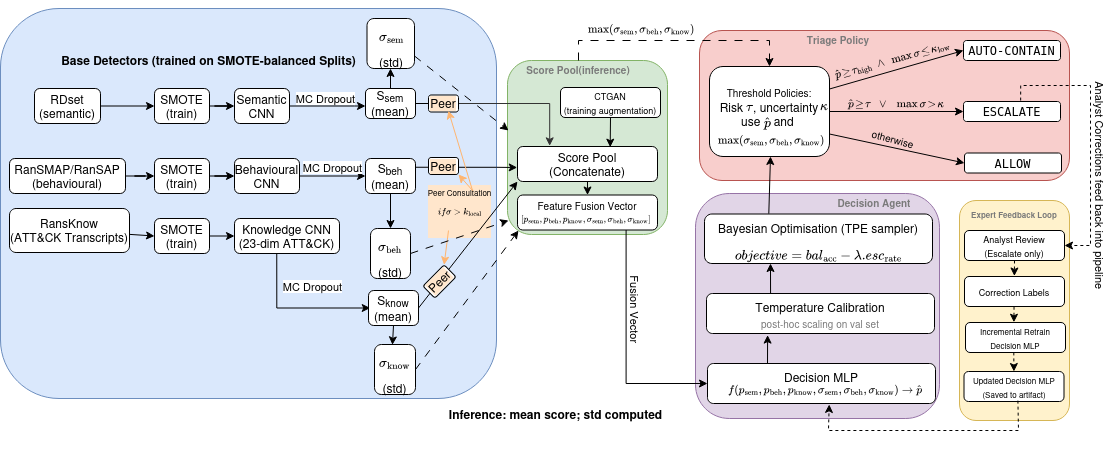
\includegraphics[width=0.78\linewidth]{fig0_pipeline.png}

\vspace{0.8em}
\raggedright
Three specialised CNN agents each produce $(\hat p_i, \sigma_i)$ via MC
Dropout. Peer Consultation substitutes an unreliable agent's probability
before the score pool is fused by the Decision MLP into a calibrated risk
$\hat p$. Bayesian TPE derives the four-threshold policy mapping
$(\hat p, \sigma_{\max})$ to \textsc{Auto-Contain}, \textsc{Escalate}, or
\textsc{Allow}; analyst corrections feed back via EWC-regularised
incremental retraining.
}
\end{columns}

\begin{columns}

% ─────────────────────────────────────────────────────────── COLUMN 1
\column{0.32}

\block{Why Existing Detectors Fall Short}{
\begin{itemize}
\setlength\itemsep{0.6em}
\item \textbf{No principled uncertainty} --- a deterministic softmax score
cannot distinguish a confident-correct prediction from a confident-wrong one.
\item \textbf{Heuristic modality fusion} --- equal-weight averaging of static
PE features and runtime telemetry discards per-modality reliability.
\item \textbf{Binary triage} --- alerting on every uncertain case overwhelms
analysts; auto-containing every uncertain case risks business disruption.
\end{itemize}
}

\block{Four Contributions}{
\begin{enumerate}
\setlength\itemsep{0.7em}
\item A \textbf{heterogeneous three-agent architecture} (Semantic, Behavioural,
Knowledge CNNs), each producing a probability \emph{and} an epistemic
uncertainty via $T{=}10$ MC Dropout passes.
\item A \textbf{Decision MLP fusion} of the six-dimensional score pool,
temperature-calibrated (ECE $0.027$), with \textbf{CTGAN} score-space
augmentation for class imbalance.
\item A \textbf{Bayesian TPE triage policy} over four jointly-optimised
thresholds, cutting escalation from $58.3\%\!\to\!30.6\%$ while raising
balanced accuracy $0.753\!\to\!0.864$.
\item \textbf{Peer Consultation} against knowledge collapse under concurrent
execution, and an \textbf{Expert Feedback Loop} (EWC) for continual
adaptation with negligible forgetting ($\Delta\text{AUPRC}{=}0.001$).
\end{enumerate}
}

\block{Datasets}{
\begin{itemize}
\setlength\itemsep{0.6em}
\item \textbf{RDset}: $138{,}047$ PE files ($96{,}724$ ransomware /
$41{,}323$ benign) --- Semantic Agent.
\item \textbf{RanSMAP}: $35{,}857$ ten-second hypervisor telemetry windows,
$1{,}776$ sessions, 15 hardware configurations, six ransomware families ---
Behavioural Agent.
\item \textbf{RansKnow} (ours): $718$ ATT\&CK-annotated threat-intelligence
transcripts --- Knowledge Agent.
\end{itemize}
\vspace{0.5em}
\textit{RDset, RanSMAP, and RansKnow are independently collected: no
executable appears in more than one dataset, so Semantic and Knowledge
contribute a fixed, label-independent corpus-mean score during RanSMAP
fusion --- only the Behavioural Agent carries per-sample signal there.}
}

\block{Limitations \& Future Work}{
\begin{itemize}
\setlength\itemsep{0.5em}
\item Concurrent benign+ransomware execution remains hard for the most
adversarial pairing (SDelete+REvil); Peer Consultation partially recovers
detection but the system still escalates rather than confidently contains.
\item RanSMAP covers families through 2022; extension to Cl0p,
BlackCat/ALPHV, LockBit 3.0 is future work.
\item An adaptive attacker could in principle suppress $\sigma_{\max}$ while
keeping $\hat p$ sub-threshold; online Bayesian recalibration of triage
thresholds under concept drift is likewise deferred to future work.
\end{itemize}
}

% ─────────────────────────────────────────────────────────── COLUMN 2
\column{0.36}

\block{Triage Policy over $(\hat p,\sigma_{\max})$ Space}{
\begin{equation*}
\pi(\hat p, \sigma_{\max};\Theta) =
\begin{cases}
\textsc{Auto-Contain} & \hat p \ge \tau_{\text{high}} \wedge \sigma_{\max}\le\kappa_{\text{low}}\\
\textsc{Escalate}     & \hat p \ge \tau \vee \sigma_{\max} > \kappa\\
\textsc{Allow}        & \text{otherwise}
\end{cases}
\end{equation*}
\centering
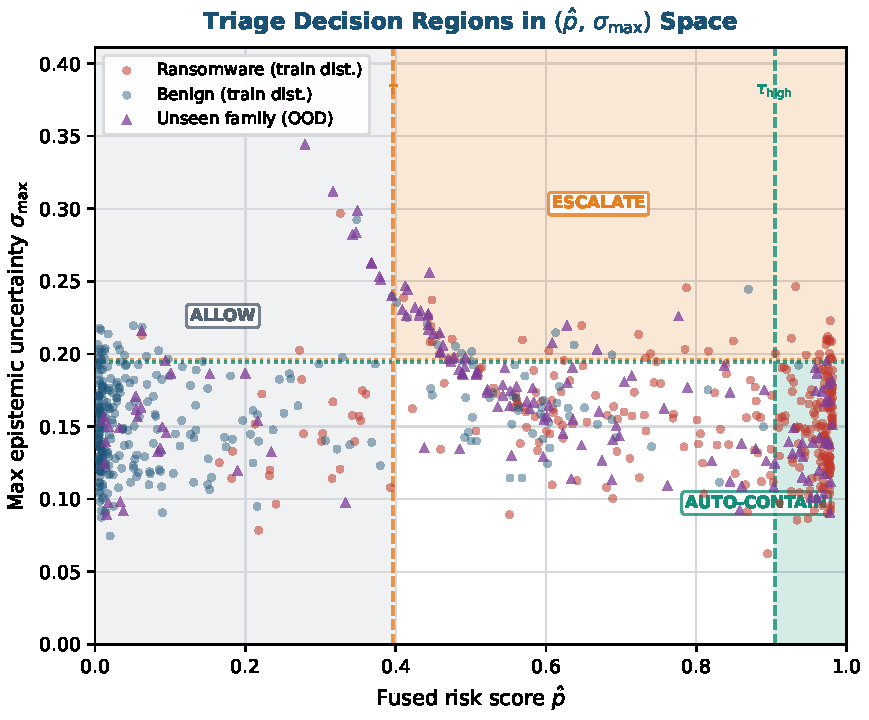
\includegraphics[width=0.85\linewidth]{fig14_triage_space.pdf}

\raggedright
\vspace{0.4em}
Out-of-distribution samples from unseen families concentrate in the
\textsc{Escalate} region ($63\%$) due to elevated $\sigma_{\max}$, converting
would-be silent misses into analyst review.
}

\block{Calibration: Fusion is a Calibration Story, not an AUROC Story}{
\centering
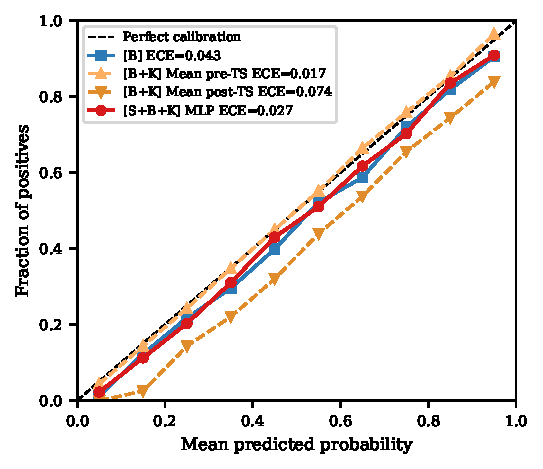
\includegraphics[width=0.85\linewidth]{fig3_calibration.pdf}

\raggedright
\vspace{0.4em}
Since Semantic/Knowledge contribute fixed corpus-mean scores on RanSMAP, the
Decision MLP cannot exceed the Behavioural Agent's own AUROC here. Its honest
value is uncertainty-gated triage: naive mean fusion is in fact better
calibrated (ECE $0.017$) than the Decision MLP (ECE $0.027$).
}

\block{Conclusion}{
A three-agent framework treating epistemic uncertainty as a
\textbf{first-class control variable} for autonomous triage: strong
in-distribution detection (AUROC $0.996$ static / $0.963$ behavioural), a
$47\%$ escalation reduction, and a Mondrian conformal wrapper giving
distribution-free coverage guarantees where exchangeability holds.
\vspace{0.4em}

\centering{\small \texttt{github.com/Henrinnes/Agentic\_SABRE}}
}

% ─────────────────────────────────────────────────────────── COLUMN 3
\column{0.32}

\block{Detection Performance}{
\centering
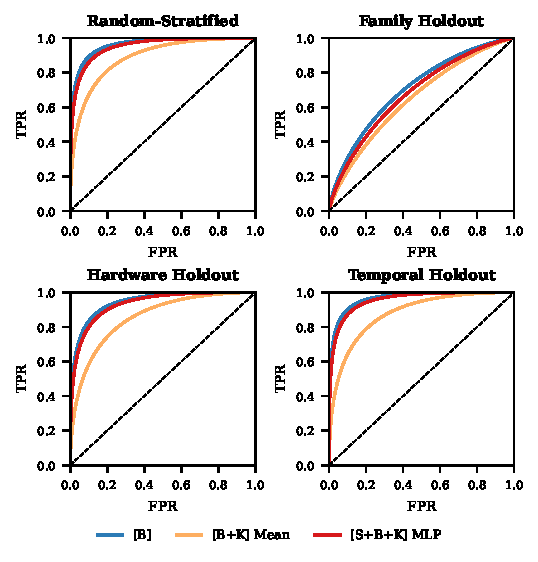
\includegraphics[width=0.95\linewidth]{fig2_roc.pdf}

\vspace{0.6em}
\begin{tabular}{lcccc}
\toprule
\textbf{System} & Random & Temporal & Family & Hardware\\
\midrule
Semantic (RDset) & \textbf{0.996} & -- & -- & --\\
Behavioural      & \textbf{0.961} & \textbf{0.960} & \textbf{0.707} & \textbf{0.939}\\
Decision MLP     & 0.952 & 0.956 & 0.681 & 0.933\\
\bottomrule
\end{tabular}
\vspace{0.4em}

\raggedright
Family holdout is the one generalisation gap: AUROC falls to $0.707$, but
elevated $\sigma_{\text{beh}}$ correctly routes most novel-family samples to
escalation rather than silent miss.
}

\block{Triage Policy Optimisation}{
\centering
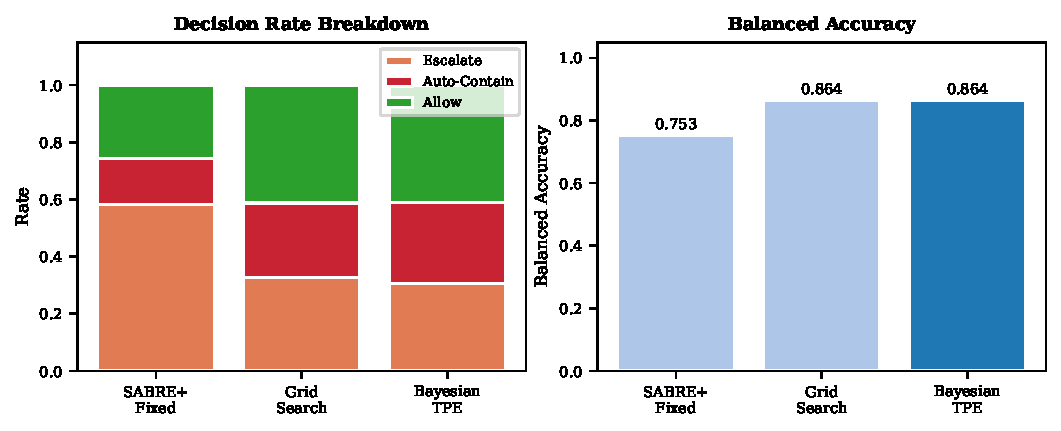
\includegraphics[width=0.95\linewidth]{fig5_policy.pdf}

\vspace{0.6em}
\begin{tabular}{lccc}
\toprule
\textbf{Policy} & Bal.\ Acc.\ $\uparrow$ & Escalate (\%) $\downarrow$ & Auto-C (\%) $\uparrow$\\
\midrule
Fixed thresholds & 0.753 & 58.3 & 16.0\\
Grid search      & 0.864 & 32.6 & 26.2\\
\textbf{Bayesian TPE} & \textbf{0.864} & \textbf{30.6} & \textbf{28.2}\\
\bottomrule
\end{tabular}
}

\block{Generalisation Across Four Splits}{
\centering
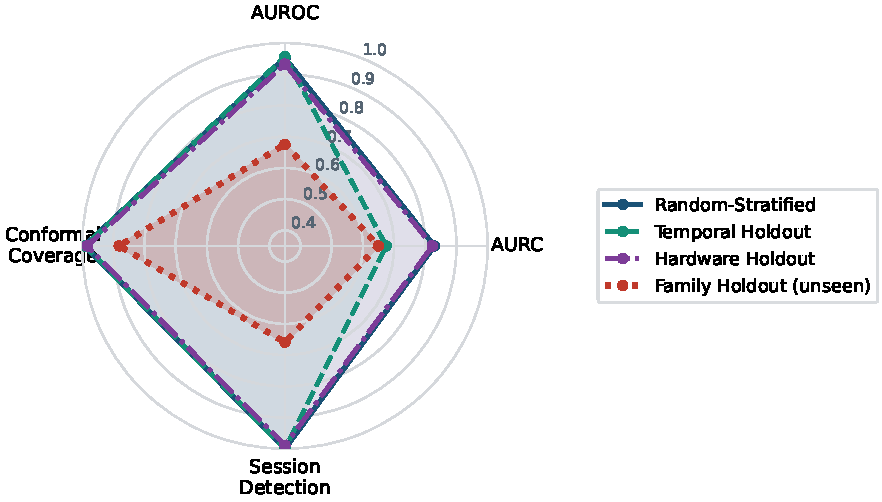
\includegraphics[width=0.75\linewidth]{fig_radar_splits.pdf}

\raggedright
\vspace{0.4em}
Random-stratified, temporal, and hardware holdout cluster tightly on every
axis; family holdout collapses inward on all four --- the same
generalisation gap, not four independent weaknesses.
}

\end{columns}

\end{document}
